% Options for packages loaded elsewhere
\PassOptionsToPackage{unicode}{hyperref}
\PassOptionsToPackage{hyphens}{url}
\PassOptionsToPackage{dvipsnames,svgnames,x11names}{xcolor}
%
\documentclass[
  letterpaper,
  DIV=11,
  numbers=noendperiod]{scrreprt}

\usepackage{amsmath,amssymb}
\usepackage{iftex}
\ifPDFTeX
  \usepackage[T1]{fontenc}
  \usepackage[utf8]{inputenc}
  \usepackage{textcomp} % provide euro and other symbols
\else % if luatex or xetex
  \usepackage{unicode-math}
  \defaultfontfeatures{Scale=MatchLowercase}
  \defaultfontfeatures[\rmfamily]{Ligatures=TeX,Scale=1}
\fi
\usepackage{lmodern}
\ifPDFTeX\else  
    % xetex/luatex font selection
\fi
% Use upquote if available, for straight quotes in verbatim environments
\IfFileExists{upquote.sty}{\usepackage{upquote}}{}
\IfFileExists{microtype.sty}{% use microtype if available
  \usepackage[]{microtype}
  \UseMicrotypeSet[protrusion]{basicmath} % disable protrusion for tt fonts
}{}
\makeatletter
\@ifundefined{KOMAClassName}{% if non-KOMA class
  \IfFileExists{parskip.sty}{%
    \usepackage{parskip}
  }{% else
    \setlength{\parindent}{0pt}
    \setlength{\parskip}{6pt plus 2pt minus 1pt}}
}{% if KOMA class
  \KOMAoptions{parskip=half}}
\makeatother
\usepackage{xcolor}
\setlength{\emergencystretch}{3em} % prevent overfull lines
\setcounter{secnumdepth}{5}
% Make \paragraph and \subparagraph free-standing
\ifx\paragraph\undefined\else
  \let\oldparagraph\paragraph
  \renewcommand{\paragraph}[1]{\oldparagraph{#1}\mbox{}}
\fi
\ifx\subparagraph\undefined\else
  \let\oldsubparagraph\subparagraph
  \renewcommand{\subparagraph}[1]{\oldsubparagraph{#1}\mbox{}}
\fi


\providecommand{\tightlist}{%
  \setlength{\itemsep}{0pt}\setlength{\parskip}{0pt}}\usepackage{longtable,booktabs,array}
\usepackage{calc} % for calculating minipage widths
% Correct order of tables after \paragraph or \subparagraph
\usepackage{etoolbox}
\makeatletter
\patchcmd\longtable{\par}{\if@noskipsec\mbox{}\fi\par}{}{}
\makeatother
% Allow footnotes in longtable head/foot
\IfFileExists{footnotehyper.sty}{\usepackage{footnotehyper}}{\usepackage{footnote}}
\makesavenoteenv{longtable}
\usepackage{graphicx}
\makeatletter
\def\maxwidth{\ifdim\Gin@nat@width>\linewidth\linewidth\else\Gin@nat@width\fi}
\def\maxheight{\ifdim\Gin@nat@height>\textheight\textheight\else\Gin@nat@height\fi}
\makeatother
% Scale images if necessary, so that they will not overflow the page
% margins by default, and it is still possible to overwrite the defaults
% using explicit options in \includegraphics[width, height, ...]{}
\setkeys{Gin}{width=\maxwidth,height=\maxheight,keepaspectratio}
% Set default figure placement to htbp
\makeatletter
\def\fps@figure{htbp}
\makeatother
\newlength{\cslhangindent}
\setlength{\cslhangindent}{1.5em}
\newlength{\csllabelwidth}
\setlength{\csllabelwidth}{3em}
\newlength{\cslentryspacingunit} % times entry-spacing
\setlength{\cslentryspacingunit}{\parskip}
\newenvironment{CSLReferences}[2] % #1 hanging-ident, #2 entry spacing
 {% don't indent paragraphs
  \setlength{\parindent}{0pt}
  % turn on hanging indent if param 1 is 1
  \ifodd #1
  \let\oldpar\par
  \def\par{\hangindent=\cslhangindent\oldpar}
  \fi
  % set entry spacing
  \setlength{\parskip}{#2\cslentryspacingunit}
 }%
 {}
\usepackage{calc}
\newcommand{\CSLBlock}[1]{#1\hfill\break}
\newcommand{\CSLLeftMargin}[1]{\parbox[t]{\csllabelwidth}{#1}}
\newcommand{\CSLRightInline}[1]{\parbox[t]{\linewidth - \csllabelwidth}{#1}\break}
\newcommand{\CSLIndent}[1]{\hspace{\cslhangindent}#1}

\KOMAoption{captions}{tableheading}
\makeatletter
\makeatother
\makeatletter
\@ifpackageloaded{bookmark}{}{\usepackage{bookmark}}
\makeatother
\makeatletter
\@ifpackageloaded{caption}{}{\usepackage{caption}}
\AtBeginDocument{%
\ifdefined\contentsname
  \renewcommand*\contentsname{Table of contents}
\else
  \newcommand\contentsname{Table of contents}
\fi
\ifdefined\listfigurename
  \renewcommand*\listfigurename{List of Figures}
\else
  \newcommand\listfigurename{List of Figures}
\fi
\ifdefined\listtablename
  \renewcommand*\listtablename{List of Tables}
\else
  \newcommand\listtablename{List of Tables}
\fi
\ifdefined\figurename
  \renewcommand*\figurename{Figure}
\else
  \newcommand\figurename{Figure}
\fi
\ifdefined\tablename
  \renewcommand*\tablename{Table}
\else
  \newcommand\tablename{Table}
\fi
}
\@ifpackageloaded{float}{}{\usepackage{float}}
\floatstyle{ruled}
\@ifundefined{c@chapter}{\newfloat{codelisting}{h}{lop}}{\newfloat{codelisting}{h}{lop}[chapter]}
\floatname{codelisting}{Listing}
\newcommand*\listoflistings{\listof{codelisting}{List of Listings}}
\makeatother
\makeatletter
\@ifpackageloaded{caption}{}{\usepackage{caption}}
\@ifpackageloaded{subcaption}{}{\usepackage{subcaption}}
\makeatother
\makeatletter
\@ifpackageloaded{tcolorbox}{}{\usepackage[skins,breakable]{tcolorbox}}
\makeatother
\makeatletter
\@ifundefined{shadecolor}{\definecolor{shadecolor}{rgb}{.97, .97, .97}}
\makeatother
\makeatletter
\makeatother
\makeatletter
\makeatother
\ifLuaTeX
  \usepackage{selnolig}  % disable illegal ligatures
\fi
\IfFileExists{bookmark.sty}{\usepackage{bookmark}}{\usepackage{hyperref}}
\IfFileExists{xurl.sty}{\usepackage{xurl}}{} % add URL line breaks if available
\urlstyle{same} % disable monospaced font for URLs
\hypersetup{
  pdftitle={Population Data Science with Python},
  pdfauthor={Yaser Khorrami; John Karuitha},
  colorlinks=true,
  linkcolor={blue},
  filecolor={Maroon},
  citecolor={Blue},
  urlcolor={Blue},
  pdfcreator={LaTeX via pandoc}}

\title{\textbf{Population Data Science with Python}}
\author{Yaser Khorrami \and John Karuitha}
\date{August 30, 2023}

\begin{document}
\maketitle
\ifdefined\Shaded\renewenvironment{Shaded}{\begin{tcolorbox}[breakable, frame hidden, sharp corners, enhanced, boxrule=0pt, borderline west={3pt}{0pt}{shadecolor}, interior hidden]}{\end{tcolorbox}}\fi

\renewcommand*\contentsname{Table of contents}
{
\hypersetup{linkcolor=}
\setcounter{tocdepth}{2}
\tableofcontents
}
\bookmarksetup{startatroot}

\hypertarget{preface}{%
\chapter*{Preface}\label{preface}}
\addcontentsline{toc}{chapter}{Preface}

\markboth{Preface}{Preface}

This is a Quarto book.

To learn more about Quarto books visit
\url{https://quarto.org/docs/books}.

\bookmarksetup{startatroot}

\hypertarget{introduction-to-python-for-data-science}{%
\chapter{\texorpdfstring{\textbf{Introduction to Python for Data
Science}}{Introduction to Python for Data Science}}\label{introduction-to-python-for-data-science}}

\hypertarget{background}{%
\section{Background}\label{background}}

In this section, we delve into the basics of Python for Data Science.
Python is a simple yet powerful programming language that has utility in
web development, scientific computing, data science and machine
learning. For a start, there are two versions of Python; Python version
2 and Python version 3. In this course, we work exclusively with Python
version 3. Moreover, our interest in this section is the use of Python
for data analysis. Let us first install Python.

\hypertarget{installing-python}{%
\section{Installing Python}\label{installing-python}}

The installation of Python will differ slightly depending on the
operating system; Windows, Mac, and Linux. The
\href{https://www.python.org/downloads/}{site}
\url{https://www.python.org/downloads/} contains the Python executables
for each operating system. ASt the time of writing this book, the Python
version release is Python 3.11.5. However, installation procedures do
not change much. The internet is full of tutorials on the installation
of Python. In this book, we refer the reader to the available
installation guidelines.

\hypertarget{installing-python-on-windows}{%
\subsection{Installing Python on
Windows}\label{installing-python-on-windows}}

Microsoft has a comprehensive set of installation procedures for
installing Python on Windows available on this
\href{https://learn.microsoft.com/en-us/windows/python/beginners}{website}
\url{https://learn.microsoft.com/en-us/windows/python/beginners}.
Microsoft recommends the installation of Python from the Microsoft
Store. We also recommend this approach because it will save you from the
complications of setting the Python path. The link also contains
information about the installation of VS Code, a popular text editor for
writing Python code. We recommend that you also install VS Code.

If you choose to download and install Python directly from the Python
Website, ensure that you set the path correctly. Specifically, when
installing Python, ensure that you tick the choice
\texttt{Add\ Python\ to\ Path} in the installation dialogue box (See
Figure 1.1).

\begin{figure}

{\centering 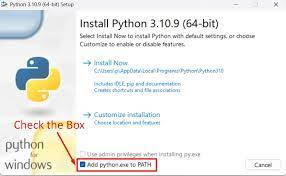
\includegraphics{"images/path.jpeg"}

}

\caption{``Add Python to Path''}

\end{figure}

\hypertarget{installing-python-on-mac-os}{%
\subsection{Installing Python on Mac
OS}\label{installing-python-on-mac-os}}

We refer the reader to the following
\href{https://www.makeuseof.com/how-to-install-python-on-mac/}{website}
\url{https://www.makeuseof.com/how-to-install-python-on-mac/} for
instructions on installing Python on Mac OS. We spewcifically point you
to the section titled ``How to Install Python With the Official
Installer'' as it offers a simpler and direct way to install Python on
Mac OS. We also recomend that the readers install VS Code by following
instructions on this
\href{https://code.visualstudio.com/docs/setup/mac}{site}
\url{https://code.visualstudio.com/docs/setup/mac}.

\hypertarget{installing-python-on-linux}{%
\subsection{Installing Python on
Linux}\label{installing-python-on-linux}}

Most linux distributions come with linux pre-installed. For instance,
Ubuntu comes with the latest Linux 3 release installed. To check the
version of Python on Linux, open the terminal and run the following
command.

\begin{verbatim}
python3 --version
\end{verbatim}

To install VS Code, follow the instructions on this
\href{https://code.visualstudio.com/docs/setup/linux}{link}
\url{https://code.visualstudio.com/docs/setup/linux}.

\hypertarget{popular-python-text-editors-and-interactive-development-environments-ides.}{%
\section{Popular Python Text Editors and Interactive Development
Environments
(IDEs).}\label{popular-python-text-editors-and-interactive-development-environments-ides.}}

There are numerous popular IDEs and text editors for use with Python.
The most popular IDE is \texttt{pycharm}. Pycharm comes in two flavors,
the professional edition and the community edition. The community
edition has reduced functionality compared to the professional edition.

The most popular text editor for Python is \texttt{VS\ Code}. VS Code is
free to download and use. This is our editor of choice iin this book.
Our choice of VS Code is out of our personal preference. You can follow
the contents of this book while using other platforms like Sublime text,
Jupyter notebooks, among others.

\hypertarget{setting-up-vs-code-for-python-programming}{%
\subsection{Setting up VS Code for Python
Programming}\label{setting-up-vs-code-for-python-programming}}

VS Code is a text editor. To make VS Code work with Python (and other
programming languages), we need to install appropriate VS Code
extensions. In our case, we install the following VS Code extensions.

\begin{itemize}
\tightlist
\item
  Python.
\item
  Jupyter
\item
  Code Runner.
\item
  Quarto
\item
  Prettier.
\end{itemize}

Let us illustrate how to install the Python extension.

\begin{itemize}
\tightlist
\item
  First, open the Extensions view (Ctrl+Shift+X).
\item
  Filter the extension list by typing `python'.
\item
  Click on the Python extension (Verify that it the extensions is
  created by Microsoft).
\item
  Finally, Install the extension (See Figure 2 and 3 below).
\end{itemize}

\begin{figure}

{\centering 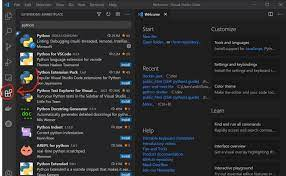
\includegraphics{"images/vs_ext.jpeg"}

}

\caption{``Open the extensions panel''}

\end{figure}

\begin{figure}

{\centering 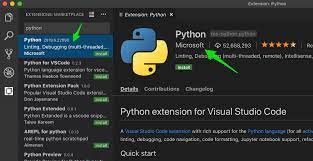
\includegraphics{"images/vs_ext_install.jpeg"}

}

\caption{``Open the extensions panel''}

\end{figure}

You can follow the same procedure to install the other extensions.

\bookmarksetup{startatroot}

\hypertarget{summary}{%
\chapter{Summary}\label{summary}}

In summary, this book has no content whatsoever.

\bookmarksetup{startatroot}

\hypertarget{references}{%
\chapter*{References}\label{references}}
\addcontentsline{toc}{chapter}{References}

\markboth{References}{References}

\hypertarget{refs}{}
\begin{CSLReferences}{0}{0}
\end{CSLReferences}



\end{document}
